\chapter{Aprendizaje por refuerzo de un controlador visual}\label{desarrollo}

En este capítulo se describe la solución desarrollada. Se detalla cómo cada una de las pequeñas partes ha tenido peso para llegar a la solución del problema. En las siguientes secciones se cubren todos estos aspectos hasta llegar a la fase de aprendizaje donde se llevarán a cabo los entrenamientos con aprendizaje por refuerzo en los diferentes entornos.

%%%%%%%%%%%%%%%%%%%%%%%%%%%%%%%%%%%%%%%%%%%%%%%%%%%%%%%%%%%%%%%%%%%%%%%%%%%%%%%%%%%%%%%%%%%%%%%%%%%%%%%%%%%%%%%%
\section{Diseño}

La estructura del proyecto está compuesta por tres grandes piezas: Gym-Gazebo, ROS y Gazebo. Como puede verse en la figura \ref{fig:project-structure} izquierda, Gym-Gazebo aparece en la parte superior del diagrama como orquestador de la información proporcionada por el simulador en primer lugar y por ROS después a través del \textit{topic}: \texttt{img\_raw} para actuar entregando los valores correspondientes al simulador a través del \textit{topic} \texttt{cmd\_vel} en orden inverso para los entrenamientos. Para situaciones que requieran reiniciar la simulación se usan los topics de Gazebo para el posicionamiento del robot en la zona deseada. Una vez se tiene el algoritmo de aprendizaje por refuerzo entrenado, se ejecuta el mismo programa pero cargando la información aprendida en la etapa anterior. A nivel estructural tiene el mismo diseño dado que se encuentra también dentro de la librería de Gym-Gazebo pero es ejecutado por otro programa. Puede verse la arquitectura en la figura \ref{fig:project-structure}  derecha.

\begin{figure}[!ht]
    \centering 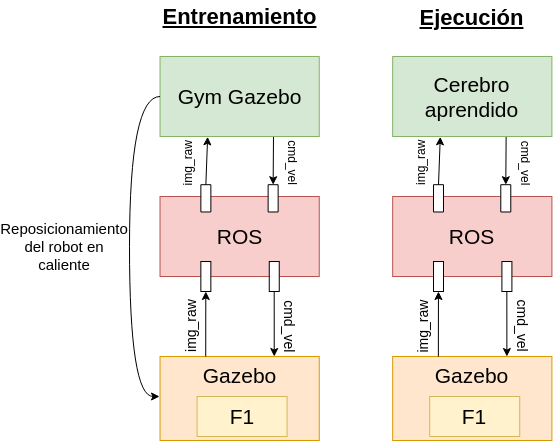
\includegraphics[width=0.5\columnwidth]{./figures/chapter_4/project-structure.png}
    \caption{
        \label{fig:project-structure}
            Estructura del proyecto.
    }
\end{figure}

Los entornos ROS y Gazebo son los encargados de representar el robot en el mundo generado con Gazebo para que sea Gym-Gazebo el que gestione y gobierne el robot.


%%%%%%%%%%%%%%%%%%%%%%%%%%%%%%%%%%%%%%%%%%%%%%%%%%%%%%%%%%%%%%%%%%%%%%%%%%%%%%%%%%%%%%%%%%%%%%%%%%%%%%%%%%%%%%%%
\section{Escenarios}\label{escenarios}

Los escenarios robóticos empleados en el proyecto para entrenar y para evaluar los cerebros aprendidos son mundos creados con el simulador Gazebo. Cada uno presenta diferentes características de longitud, número de curvas y rectas que pueden resumirse en la tabla \ref{caracteristicas-circtuitos}.

\begin{table}[ht!]
    \centering
\begin{tabular}{|l|c|c|c|c|}
\hline
\rowcolor[HTML]{EFEFEF} 
\textbf{Circuito}                            & \textbf{metros} &\Lsh & \uparrow & \Rsh \\ \hline
\cellcolor[HTML]{EFEFEF}\textbf{Simple}      & 465             & 4          & 5          & 5          \\ \hline
\cellcolor[HTML]{EFEFEF}\textbf{Nürburgring} & 597             & 6          & 9          & 8          \\ \hline
\cellcolor[HTML]{EFEFEF}\textbf{Montreal}                 & 1563            & 7          & 9          & 9          \\ \hline
\end{tabular}
\caption{Características de los circuitos.}\label{caracteristicas-circtuitos}
\end{table}


Puede verse una vista cenital de los circuitos (figura \ref{fig:gazebo-circuitos}) donde la complejidad de cada uno es diferente. El <<circuito simple>> (figura \ref{fig:gazebo-simple-circuit}) es un recorrido sintético que se utiliza en la plataforma RoboticsAcademy\footnote{\url{https://github.com/JdeRobot/RoboticsAcademy}} para ejercicios de navegación de robots. Las curvas son de complejidad baja y generalmente abiertas. En las réplicas de los circuitos reales de Fórmula-1 de <<Nürburgring>> (figura \ref{fig:gazebo-nurburgring}) y <<Montreal>> (figura \ref{fig:gazebo-montreal}) vemos que existen curvas más cerradas, cambios bruscos en mitad de una curva o pequeños \textit{zig-zags} que ponen a prueba los límites del algoritmo para situaciones con cambios más repentinos.

\begin{figure}[ht!]
  \begin{center}
    \subfloat[Circuito simple.]{\label{fig:gazebo-simple-circuit}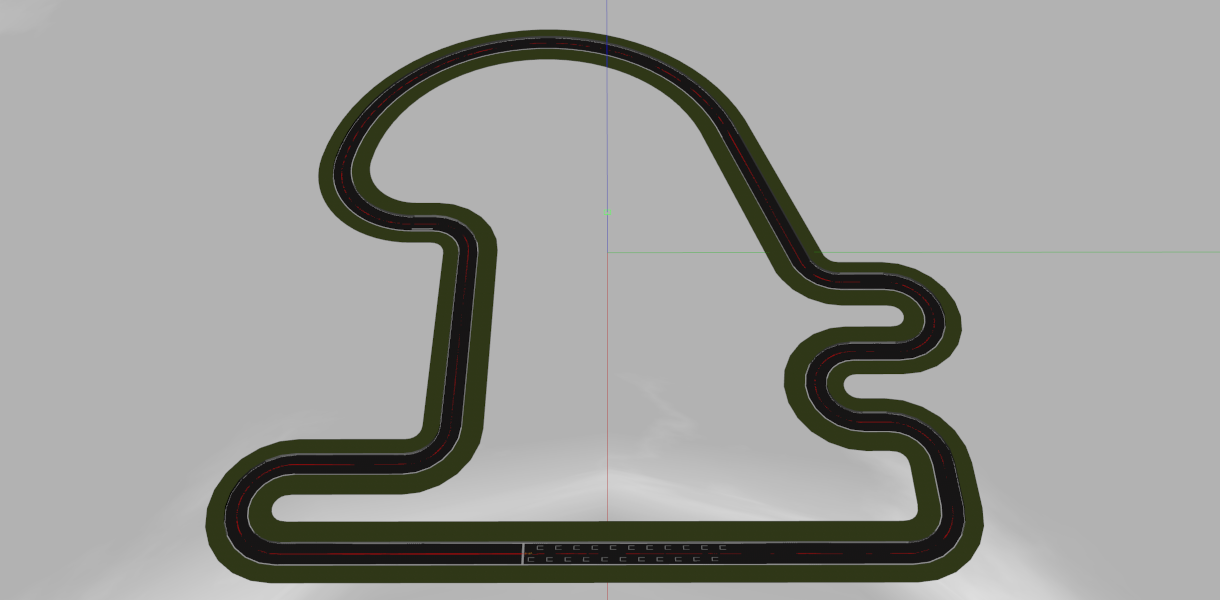
\includegraphics[width=.332\linewidth]{figures/chapter_4/circuit-simple-circuit.png}}
    \hspace{0.1cm}
    \subfloat[Nürburgring.]{\label{fig:gazebo-nurburgring}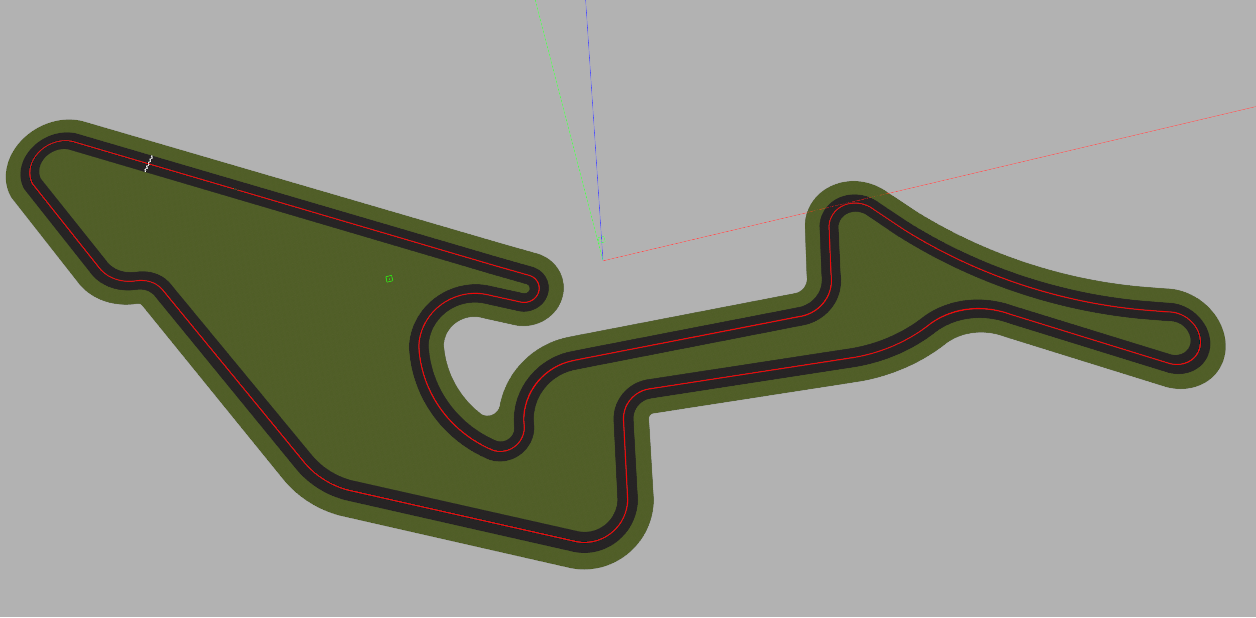
\includegraphics[width=.32\linewidth]{figures/chapter_4/circtuit-nurburgring.png}}
    \hspace{0.1cm}
    \subfloat[Montreal.]{\label{fig:gazebo-montreal}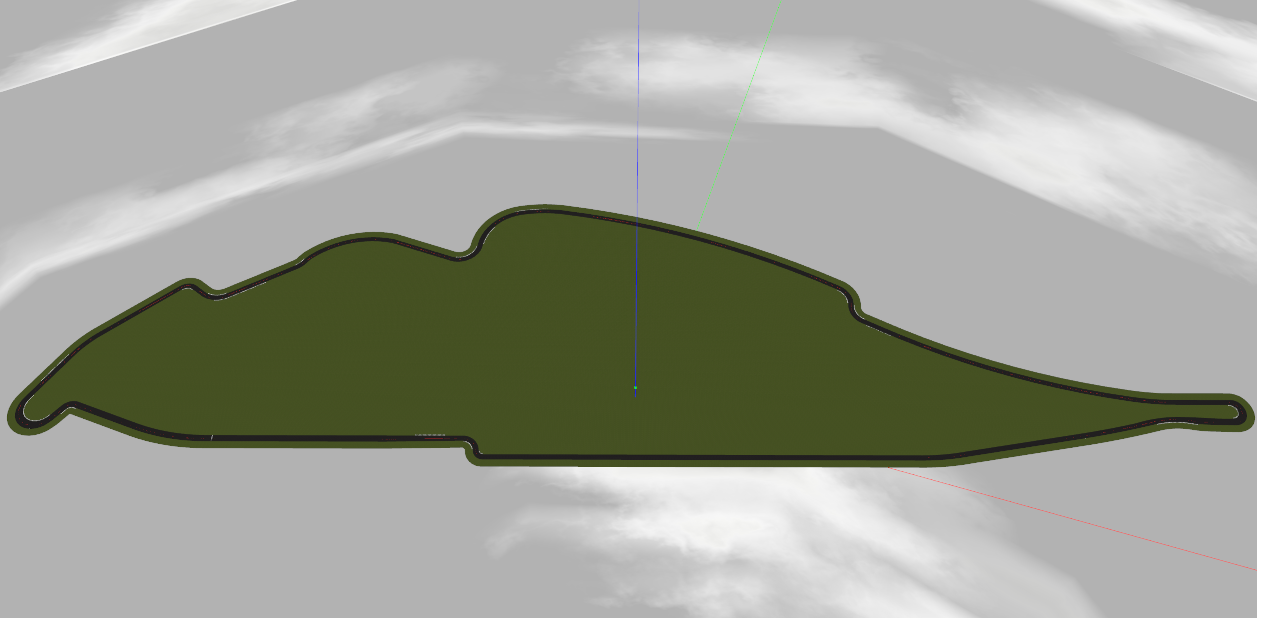
\includegraphics[width=.32\linewidth]{figures/chapter_4/circuit-montreal.png}}
  \end{center}
  \centering
  \captionsetup{justification=centering,margin=2cm}
  \caption{Escenarios de Gazebo.}
  \label{fig:gazebo-circuitos}
\end{figure}


En todos ellos se utiliza el mismo modelo de coche basado en un Fórmula-1 (figura \ref{fig:f1-model}). El modelo del coche cuenta con una cámara situada en la parte delantera como sensor principal.

\begin{figure}[!ht]
    \centering 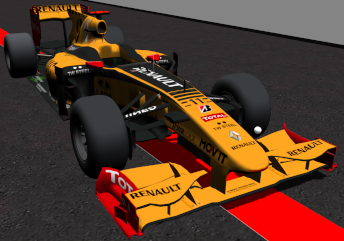
\includegraphics[width=0.4\columnwidth]{./figures/chapter_4/model_f1.png}
    \caption{
        \label{fig:f1-model}
            Modelo de Fórmula-1 empleado en el entrenamiento.
    }
\end{figure}

Se capturan imágenes a unos 20 fotogramas por segundo (fps) y está equipado con un sensor láser de distancia, pero no se usará en este TFM dado que está más enfocado en un control estrictamente basado en visión. Los motores del coche se gobiernan comandándoles continuamente la velocidad de avance deseada $v (m/s)$ y la velocidad de giro deseada $w (rad/s)$.

%%%%%%%%%%%%%%%%%%%%%%%%%%%%%%%%%%%%%%%%%%%%%%%%%%%%%%%%%%%%%%%%%%%%%%%%%%%%%%%%%%%%%%%%%%%%%%%%%%%%%%%%%%%%%%%%
\section{Adaptación de Gym-Gazebo}\label{adaptacion-gym-gazebo}

La librería principal desde donde se gestionan todos los entornos y comportamientos así como el registro de los resultados una vez finalizados los experimentos es Gym-Gazebo. Para el desarrollo de este proyecto se ha modificado la librería por fases y agregado un nuevo ejercicio entrenable al repertorio: la conducción autónoma usando una cámara como sensor. Para este nuevo ejercicio del <<gimnasio>> se han creado varios escenarios (mencionados en el punto \ref{escenarios}) con diferentes complejidades que enriquecen el conjunto de pruebas.\\

Para la resolución el ejercicio se crea un nuevo agente, el Fórmula-1, que tiene asociado un entorno (en términos de la librería OpenAI Gym, un \textit{environment}) que es donde se realizan los cálculos y se evalúa cada paso (o \textit{step}) que se da en el circuito. En él se describen los mismos métodos que en el resto de entornos de la librería pero con diferentes operaciones en su interior, adaptadas al ejercicio en cuestión.\\

La biblioteca incluye todos los ingredientes de un aprendizaje por refuerzo y se encarga de reinicia al simulador Gazebo y/o la posición del robot en el escenario simulado cuando es necesario.\\

No ha sido posible la incorporación al repositorio original de Gym-Gazebo de todas las mejoras creadas para el proyecto como son: la creación del nuevo ejercicio, los escenarios, entornos, mundos de Gazebo, modelos, etc, dado que el repositorio oficial de la librería se encuentra bloqueado. Actualmente todas las mejoras sí se encuentran integradas en el repositorio del Trabajo Fin de Máster\footnote{\url{https://github.com/RoboticsLabURJC/2019-tfm-ignacio-arranz/tree/master/gym-gazebo}}.

%%%%%%%%%%%%%%%%%%%%%%%%%%%%%%%%%%%%%%%%%%%%%%%%%%%%%%%%%%%%%%%%%%%%%%%%%%%%%%%%%%%%%%%%%%%%%%%%%%%%%%%%%%%%%%%%
\subsection{Aprendizaje por refuerzo con Gym-Gazebo}

Para la creación de ejercicios con algoritmos de aprendizaje por refuerzo dentro de la librería Gym-Gazebo es necesario crear una serie de métodos obligatorios, ya que esta biblioteca actúa de intermediaria entre el software robótico (ROS y Gazebo) y la librería de OpenAI Gym. La estandarización que creó OpenAI Gym donde se unificaban todos los ejercicios del gimnasio bajo una misma estructura de métodos definida se hereda también en Gym-Gazebo. Los métodos más relevantes para la ejecución de un ejercicio en Gym-Gazebo son:\\

\begin{itemize}
    \item \textbf{Método} \texttt{step}: Es uno de los métodos más importantes de la librería y es donde se programa la lógica del robot en cada paso que da. Recibe como parámetro de entrada una acción que ejecuta (da un paso) y analiza el entorno con los sensores (cámara, láser, etc), buscando características en él y generando una recompensa acorde en función de una serie de condiciones. Este método devuelve el estado siguiente $s_t+1$ (\texttt{state}), la recompensa (\texttt{reward}), la variable booleana \texttt{done} indicando si se sigue la ejecución o hay que reiniciar y un parámetro opcional (\texttt{info}) con información adicional.\\
    \item \textbf{Método} \texttt{reset}: Es otro de los métodos importantes de todo algoritmo de aprendizaje por refuerzo y representa el retorno del agente a la posición inicial del entorno, el reinicio. Este método ocurre cuando en el método \texttt{step} se ha dado una condición que impide seguir avanzando, por ejemplo, el robot se ha chocado. El retorno a la posición de origen calcula también el nuevo estado de partida $s_t$ desde el cual comenzará a llamarse al método \texttt{step}.\\
    \item \textbf{Métodos} \texttt{pause} y \texttt{unpause}: Al inicio de cada paso o reinicio generado por los métodos anteriores es necesario detener la simulación de Gazebo durante un instante para generar el estado siguiente ($s+1$) para evaluar lo recogido por los sensores en un instante y evitar sobrecarga en el código y en el robot y tener que desechar alguna lectura. Una vez calculados se llama al método \texttt{unpause} para reanudar de nuevo la ejecución.\\
\end{itemize}

Con estos métodos definidos, se tiene una estructura que permite crear ejercicios que resuelvan situaciones utilizando algoritmos de aprendizaje por refuerzo. El proceso de modificación de Gym-Gazebo hasta crear el ejercicio principal que resuelve este Trabajo Fin de Máster ha seguido una serie de fases que se detallan a continuación.

%%%%%%%%%%%%%%%%%%%%%%%%%%%%%%%%%%%%%%%%%%%%%%%%%%%%%%%%%%%%%%%%%%%%%%%%%%%%%%%%%%%%%%%%%%%%%%%%%%%%%%%%%%%%%%%%
\subsection{Fase 1: Sorteo de obstáculos con sensor de distancia y robot \textit{TurtleBot}}

Para la construcción del entorno deseado (mundos, modelo y cámara como sensor), se partió inicialmente de un ejercicio con el que contaba la librería de Gym-Gazebo en el que un robot \textit{Turtlebot} avanzaba por un laberinto sin colisionar con las paredes usando el sensor del láser, como puede verse en la figura \ref{fig:turtlebot-laser}.

\begin{figure}[!ht]
    \centering 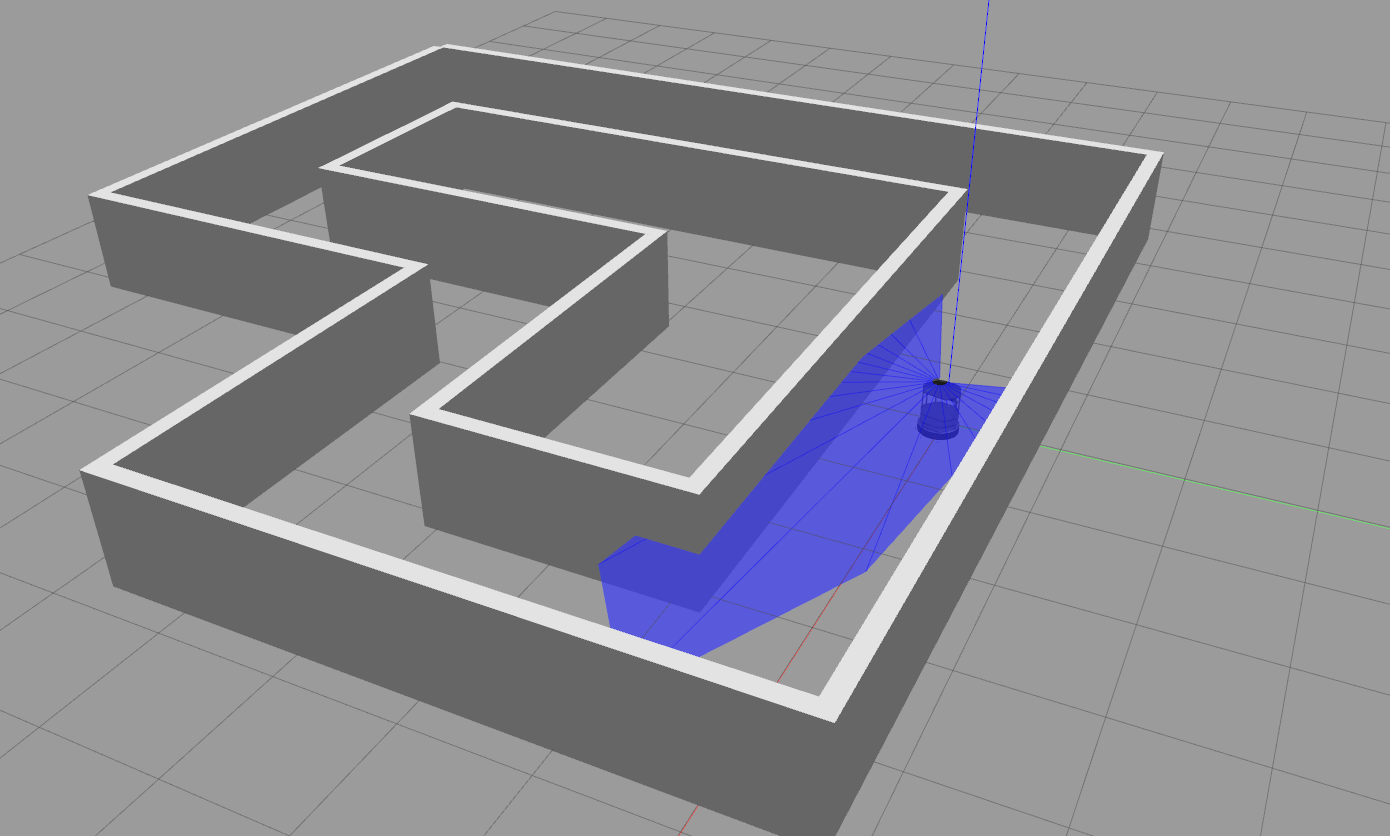
\includegraphics[width=0.4\columnwidth]{./figures/chapter_4/turtlebot_laser.png}
    \caption{Robot \textit{Turtlebot} con el sensor láser en el laberinto.\label{fig:turtlebot-laser}}
\end{figure}

Este robot, pasados una serie de episodios conseguía circular por el laberinto por el centro del pasillo evitando colisionar. Este ejercicio es la base para construir la solución a la navegación basada en visión dado que el objetivo de ambos es el mismo, evitar colisionar con la pared siguiendo un carril.\\

Este ejercicio consiguió replicarse con éxito desde la última versión congelada de la biblioteca y ejecutándose en un sistema operativo más moderno.

%%%%%%%%%%%%%%%%%%%%%%%%%%%%%%%%%%%%%%%%%%%%%%%%%%%%%%%%%%%%%%%%%%%%%%%%%%%%%%%%%%%%%%%%%%%%%%%%%%%%%%%%%%%%%%%%
\subsection{Fase 2: Sorteo de obstáculos con sensor de distancia y un Fórmula-1}

Un segundo paso para adaptar la biblioteca Gym-Gazebo a la aplicación de control visual ha sido replicar las condiciones del ejercicio del \textit{Turtlebot} pero con el mundo del <<Circuito Simple>>, con el modelo del Fórmula-1 como agente y manteniendo el láser como sensor. Puede verse el resultado de trasladar la configuración del \textit{Turtlebot} al Fórmula-1 en la figura \ref{fig:f1-laser}.

\begin{figure}[!ht]
    \centering 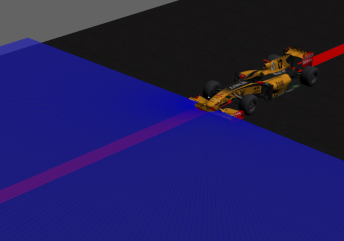
\includegraphics[width=0.5\columnwidth]{./figures/chapter_4/model_f1_laser.png}
    \caption{Fórmula-1 con el sensor láser en el circuito simple.\label{fig:f1-laser}}
\end{figure}

El objetivo de esta variante era completar el circuito sin colisionar con las paredes. En este caso la línea roja, pese a estar encima de la carretera era ignorada y únicamente se hacía un cálculo del centro a través de los haces del láser dividiendo el barrido de 180 medidas láser en 5 sectores, como se puede ver en el fragmento \ref{lst:calculo-centro-laser}.

\vspace{5mm}

\begin{tabular}{c}
\begin{lstlisting}[basicstyle=\ttfamily\scriptsize, caption={Cálculo del centro del carril usando el láser.}, captionpos=b, numbers=none, label={lst:calculo-centro-laser}, style=Python]
laser_len = len(data.ranges)
left_sum = sum(data.ranges[laser_len - (laser_len / 5):laser_len - (laser_len / 10)])
right_sum = sum(data.ranges[(laser_len / 10):(laser_len / 5)])

center_detour = (right_sum - left_sum) / 5
\end{lstlisting}
\end{tabular}

\vspace{5mm}

Los actuadores para el modelo del Fórmula-1 son los mismos que se utilizan en el ejercicio del \textit{Turtlebot}, velocidad lineal $(m/s)$ y velocidad angular $(rad/s)$. En este sentido, la adaptación al Fórmula-1 ha sido directa.

%%%%%%%%%%%%%%%%%%%%%%%%%%%%%%%%%%%%%%%%%%%%%%%%%%%%%%%%%%%%%%%%%%%%%%%%%%%%%%%%%%%%%%%%%%%%%%%%%%%%%%%%%%%%%%%%
\subsection{Fase 3: Información visual}

Con la variante del ejercicio con el sensor láser resolviendo el entorno satisfactoriamente el tercer paso fue cambiar ese sensor por la cámara para entrenar con información visual, registrando y creando el escenario en el fichero de entornos, como puede verse en el fragmento \ref{lst:registro-ejercicio-gym-gazebo}.\\

\vspace{5mm}

\begin{tabular}{c}
\begin{lstlisting}[basicstyle=\ttfamily\footnotesize, caption={Registro de un nuevo entorno en Gym-Gazebo.}, captionpos=b, numbers=none, label={lst:registro-ejercicio-gym-gazebo}, style=Python]
register(
    id='GazeboF1QlearnCameraEnv-v0',
    entry_point='gym_gazebo.envs.f1:GazeboF1QlearnCameraEnv',
)
\end{lstlisting}
\end{tabular}

\vspace{5mm}

El cambio del sensor láser a la cámara es un cambio sencillo debido a la modularidad del código de Gym-Gazebo. Para la captura de la imagen del entorno se crea un bucle en el método \texttt{step} que itera hasta tener una imagen en el \textit{buffer} de imágenes para poder extraer. Para convertir los datos en bruto que se captan desde el sensor se utiliza la librería de ROS \texttt{cv\_bridge}. Esta biblioteca convierte los datos a matrices que las librerías de OpenCV y Numpy pueden entender. Puede verse el código en el fragmento \ref{lst:captura-imagen-gym-gazebo}.\\

\vspace{5mm}

\begin{tabular}{c}
\begin{lstlisting}[basicstyle=\ttfamily\scriptsize, caption={Extracción de la imagen tomada desde la cámara.}, captionpos=b, numbers=none, label={lst:captura-imagen-gym-gazebo}, style=Python] 
while not image_data or not success:
    image_data = rospy.wait_for_message('/F1ROS/cameraL/image_raw', Image, timeout=5)
    cv_image = CvBridge().imgmsg_to_cv2(image_data, "bgr8")
    f1_image_camera = self.image_msg_to_image(image_data, cv_image)
    if f1_image_camera:
        success = True
\end{lstlisting}
\end{tabular}

\vspace{5mm}

%%%%%%%%%%%%%%%%%%%%%%%%%%%%%%%%%%%%%%%%%%%%%%%%%%%%%%%%%%%%%%%%%%%%%%%%%%%%%%%%%%%%%%%%%%%%%%%%%%%%%%%%%%%%%%%%
\subsection{Fase 4: Reinicios aleatorios}

Otro elemento añadido a la librería Gym-Gazebo es la posibilidad de hacer reinicios aleatorios en unos puntos seleccionados del circuito. El motivo de esta mejora es acelerar el entrenamiento dándole al agente situaciones que solo se encontrará cuando complete parte del circuito. Para casos en los que la convergencia no es tan rápida permite al agente aprender de una manera más ágil en la etapa inicial del entrenamiento donde la capacidad de exploración está todavía muy viva. Sin estos reinicios, si al final del recorrido hay una situación que nunca ha explorado y requiere reiniciar el episodio necesitará recorrer de nuevo todo el circuito para volver a encontrarse esa situación.\\

Los escenarios donde el agente entrena son: el <<Circuito Simple>> y Nürburgring. Para ambos, se ha creado un conjunto de posiciones desde las cuales se considera que se cubren estas necesidades. En la figura \ref{fig:reinicios-simple} pueden verse las posiciones de reinicio para el <<Circuito Simple>> así como la dirección que toma el vehículo en esa posición. En algunos casos se invierte el sentido para enriquecer aún más el repertorio y balancear el número de curvas.

\begin{figure}[!ht]
    \centering 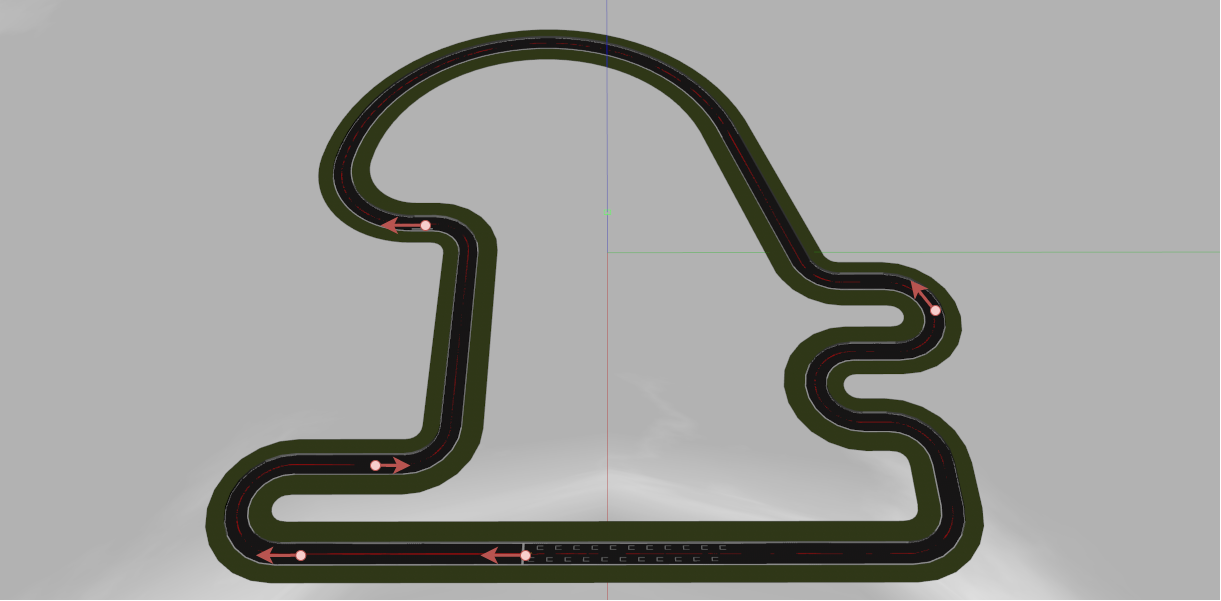
\includegraphics[width=0.8\columnwidth]{./figures/chapter_4/circuito_simple_reinicios.png}
    \caption{Posiciones del circuito simple}\label{fig:reinicios-simple}
\end{figure}

De igual manera, pueden verse los puntos de reinicio donde el agente se posicionará para el circuito de Nürburgring en la figura \ref{fig:reinicios-nurburgring}.

\begin{figure}[!ht]
    \centering 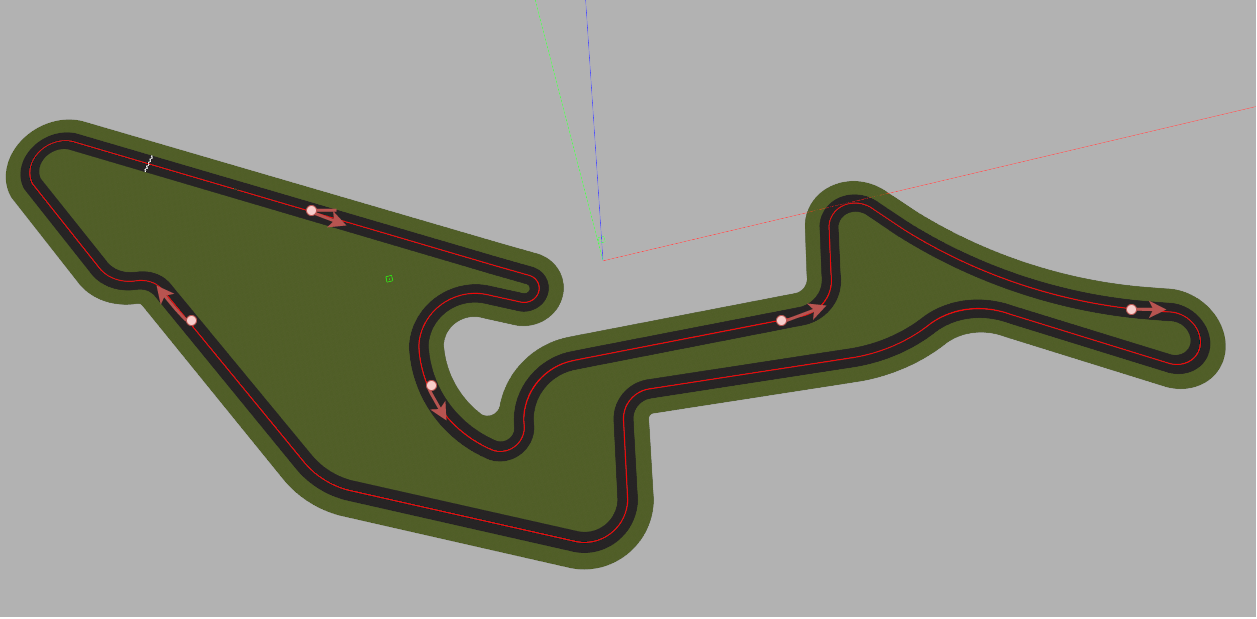
\includegraphics[width=0.8\columnwidth]{./figures/chapter_4/nurburgring_reinicios.png}
    \caption{Posiciones de Nürburgring}\label{fig:reinicios-nurburgring}
\end{figure}

%%%%%%%%%%%%%%%%%%%%%%%%%%%%%%%%%%%%%%%%%%%%%%%%%%%%%%%%%%%%%%%%%%%%%%%%%%%%%%%%%%%%%%%%%%%%%%%%%%%%%%%%%%%%%%%%
%%%%%%%%%%%%%%%%%%%%%%%%%%%%%%%%%%%%%%%%%%%%%%%%%%%%%%%%%%%%%%%%%%%%%%%%%%%%%%%%%%%%%%%%%%%%%%%%%%%%%%%%%%%%%%%%
\section{Entrenamiento}

Con las modificaciones realizadas sobre la librería y el nuevo ejercicio entrenable integrado en Gym-Gazebo se elabora un plan de entrenamiento que tendrá en cuenta principalmente dos factores: el \textit{número de percepciones} y el \textit{número de acciones}.

%%%%%%%%%%%%%%%%%%%%%%%%%%%%%%%%%%%%%%%%%%%%%%%%%%%%%%%%%%%%%%%%%%%%%%%%%%%%%%%%%%%%%%%%%%%%%%%%%%%%%%%%%%%%%%%%
\subsection{Algoritmo Q-Learning}\label{qlearning}

En el núcleo del problema se encuentra el algoritmo encargado de recibir los pares $(estado, acción)$ que retorna la librería de Gym-Gazebo y almacenar la $recompensa$ asociada para rellenar la <<Tabla-Q>> que contenga todas las situaciones que ha visto. Esta tabla contiene el par (\textit{estado, acción}) como clave y el valor de la \textit{recompensa} como valor. Este sistema de registro encaja muy bien en los controladores reactivos para gobernar el comportamiento de robots. Puede verse el flujo de registro en la tabla en la figura \ref{fig:qlearning-grafica}.\\

\begin{figure}[!ht]
    \centering 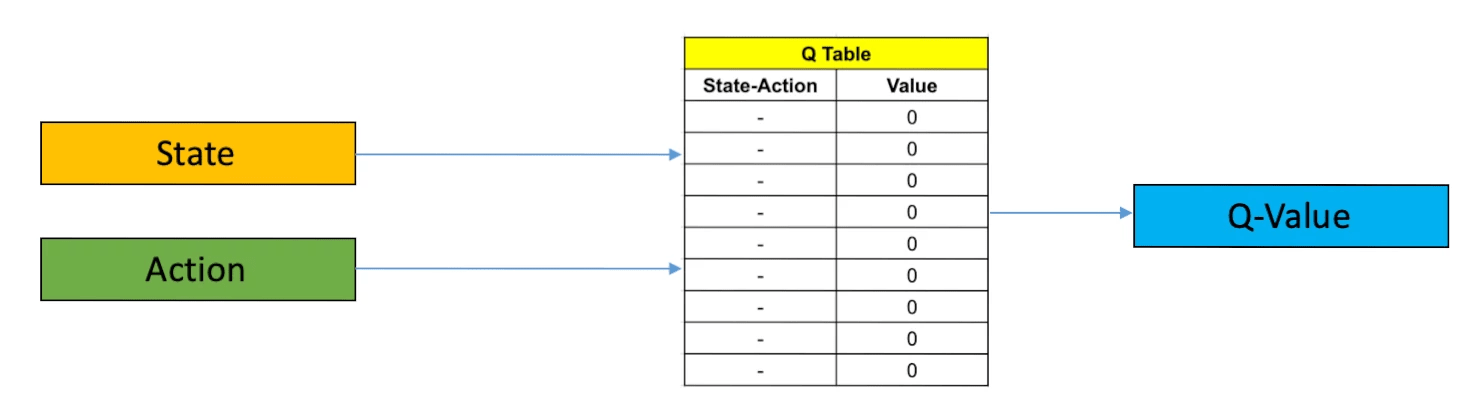
\includegraphics[width=0.8\columnwidth]{./figures/chapter_4/qlearning-dqn.png}
    \caption{Estructura de Q-Learning}\label{fig:qlearning-grafica}
\end{figure}


En este trabajo se utiliza el algoritmo Q-Learning. Es un algoritmo de aprendizaje muy usado para la resolución de problemas con entornos no modelados. En general el algoritmo converge muy rápido, es eficiente, funciona a través de las observaciones que realiza el agente durante el entrenamiento y es relativamente sencilla su implementación. Estas características hacen que encaje perfectamente con el problema de control visual que se quiere solucionar.\\

Durante el entrenamiento al robot se le presentan diferentes situaciones (\textit{estados}), el algoritmo va probando posibles actuaciones (\textit{acciones}) como respuesta a ellas y va recogiendo las recompensas observadas en el simulador robótico a esas combinaciones. El resultado neto es que el algoritmo aprende una Tabla-Q, $Q(s,a)$, que contiene cuál es la mejor respuesta para cada situación a la luz de lo experimentado durante el entrenamiento. A mayor número de pares (\textit{estado, acción}) se tiene una mayor Tabla-Q con más posibilidades. Esto tiene como contrapartida que, a mayor número de acciones mayor complejidad para resolver el problema y mayor tiempo de entrenamiento hasta la convergencia.\\

La ecuación que define el comportamiento de este algoritmo es la siguiente:

\begin{mycapequ}
   \begin{equation}
     Q(s,a) \leftarrow (1 - \alpha) Q_{s,a} + \alpha(r + \gamma \cdot \max_{a'}Q_{s',a'})
   \end{equation}
   \caption{Ecuación de Q-Learning}\label{ecuacion-qlearning}
\end{mycapequ}

Donde:\\
\begin{itemize}
    \item $\alpha (0 < \alpha \leq 1) \rightarrow$ es el índice de aprendizaje o \textit{learning rate}. Si $\alpha = 0,$ $Q(s, a)$ nunca es actualizada y, por tanto, no se produce aprendizaje. Por el contrario si $\alpha = 1, Q(s,a)$ se actualiza lo máximo posible en cada iteración. Aunque pueda parecer tentador, tener un valor de $\alpha = 1$ implica que el resultado puede olvidar lo que ha ido aprendiendo en etapas anteriores. Es necesario tener un ajuste en este parámetro para equilibrar ambas situaciones. Para este proyecto se selecciona el valor de $\alpha = 0.8$ por ser el más equilibrado.\\
    \item $r \rightarrow$ o \textit{recompensa} (\textit{reward)} es el valor devuelto como consecuencia de tomar una acción y pasar del estado $s_t$ al estado $s_{t+1}$.\\
    \item $\gamma (0 < \gamma \leq 1) \arrowright$ es el factor de descuento (\textit{discount factor}) que relaciona acciones y recompensas a largo plazo (\textit{long term reward}). Es un valor que consigue relacionar si una secuencia de acciones dará como resultado una mayor recompensa, actuando como una <<memoria>> para dar más valor a las recompensas anteriores que a las futuras. Entra dentro también de este ámbito más psicológico de esta rama del aprendizaje donde la experiencia te asegura un estado y lo que está por venir es desconocido. Se puede interpretar como la probabilidad de tener éxito en cada paso que se toma.\\
\end{itemize}

Un entrenamiento utilizando el algoritmo de Q-Learning sigue la siguiente secuencia hasta conseguir la convergencia:\\

\begin{enumerate}
    \item Se comienza con la tabla Q vacía para $Q(s,a)$.\\
    \item Se obtiene de un paso (\textit{step}) los valores: estado, acción, recompensa y estado siguiente $(s, a, r, s')$. En este paso se decide qué acción se toma, atendiendo a las condiciones de exploración o explotación.\\
    \item Se actualiza la ecuación de Bellman: $Q(s,a) \leftarrow (1 - \alpha) Q_{s,a} + \alpha(r + \gamma \cdot \max_{a'}Q_{s',a'})$.\\
    \item Se comprueban las condiciones de convergencia. Si no se cumplen se vuelve al paso 2.\\
\end{enumerate}

Cabe destacar del procedimiento anterior el paso 2. Durante el entrenamiento se lleva a cabo un proceso de exploración del entorno, representado como una cadena de Markov. Durante esta etapa el algoritmo irá tomando aleatoriamente acciones que le llevan a descubrir los límites de sus posibilidades. Este valor viene representado por el parámetro \textit{epsilon} ($\epsilon$) que en los inicios del entrenamiento tiene un valor cercano a $1$. En el fragmento \ref{lst:select_action} de código puede verse como inicialmente se depende de un valor aleatorio muy alto para que se obtenga de la Tabla-Q la mejor recompensa:\\

\vspace{5mm}

\begin{tabular}{c}
\begin{lstlisting}[basicstyle=\ttfamily\scriptsize, caption={Selección de acciones: exporación vs explotación.}, captionpos=b, numbers=none, label={lst:select_action}, style=Python] 
q = [self.getQValues(state, a) for a in self.actions]
maxQ = max(q)

if random.random() < self.epsilon:
    minQ = min(q)
    mag = max(abs(minQ), abs(maxQ))
    # add random values to all the actions, recalculate maxQ
    q = [q[i] + random.random() * mag - .5 * mag for i in range(len(self.actions))] 
    maxQ = max(q)

count = q.count(maxQ)
if count > 1:
    best = [i for i in range(len(self.actions)) if q[i] == maxQ]
    i = random.choice(best)
else:
    i = q.index(maxQ)

action = self.actions[i] 
\end{lstlisting}
\end{tabular}

\vspace{5mm}

A medida que el entrenamiento avanza y se va paulatinamente completando la tabla $Q(s,a)$ (el vehículo se encuentra con nuevas situaciones), el valor de $\epsilon$ disminuye. Cuando este parámetro es lo suficientemente bajo las acciones que tomará el agente ya no son aleatorias sino que buscará en la tabla aquellas que retornan la máxima recompensa.\\

Este elemento es una pieza muy importante dentro del algoritmo dado que da al agente la posibilidad de ejecutar acciones que no retornan la mejor recompensa pero le permite actualizar estados no explorados de $Q(s,a)$ para después, en la etapa de explotación, reforzar y perfeccionar aquellas combinaciones de $(estado, acción)$ que retornan mejores valores. Esta política se le conoce como política codiciosa o \textit{epsilon-greedy}.\\

En la mejora añadida a la librería de Gym-Gazebo este parámetro \textit{epsilon} comienza con un valor de $0.99$ y en cada episodio se le aplica un factor de descuento de 0.998 que lo hace disminuir paulatinamente. En entrenamientos donde el número de episodios es pequeño dado que consigue estar mucho tiempo sobre la línea roja, este factor se aplica cada 1000 pasos (\texttt{steps}) que es, aproximadamente, una cuarta parte del circuito. Este factor de descuento añade la posibilidad de que el agente pueda en un mismo entrenamiento explorar (reconocer el mayor número de estados o situaciones posible) y explotar (ajustar los valores de las situaciones conocidas).\\

Con todos estos elementos solo se necesita conocer qué conjunto de (\textit{estado, acción}) devuelve mejores recompensas así como el conjunto de valores óptimo de \textit{alpha} (tasa de aprendizaje), \textit{gamma} (factor de descuento) y \textit{epsilon} (para medir el grado de explotación y exploración) que configura el mejor entrenamiento y posterior ejecución.\\

Siendo esta la estructura general del algoritmo Q-Learning hay que describir las concreciones necesarias para aplicarlo al problema de conducción autónoma, del control visual deseable: 
\begin{enumerate}
    \item Los estados son las percepciones simplificadas desde la imagen obtenida por la cámara del coche,
    \item las acciones son las actuaciones posibles sobre los motores,
    \item la recompensa habrá que definirla y,
    \item habrá que dar unos valores razonables a los parámetros de aprendizaje \textit{alfa}, \textit{gamma} y \textit{epsilon}.
\end{enumerate}


%%%%%%%%%%%%%%%%%%%%%%%%%%%%%%%%%%%%%%%%%%%%%%%%%%%%%%%%%%%%%%%%%%%%%%%%%%%%%%%%%%%%%%%%%%%%%%%%%%%%%%%%%%%%%%%%
\subsection{Percepción simplificada}\label{percepcion-simplificada}

El objetivo del vehículo es conducir de manera autónoma por encima de la línea roja dibujada en el asfalto del circuito dada una imagen a través de la cámara situada encima. Esta imagen de entrada tiene unas dimensiones de $640x480$ píxeles en formato BGR (disposición típica de los canales de color en la librería de OpenCV).\\

Un ejemplo de esta imagen de entrada en una recta puede verse en la figura \ref{fig:simple-image}. Esta imagen contiene mucha información pero no toda ella es valiosa. La parte de interés se encuentra en la mitad inferior, donde están la línea roja y el asfalto. En esta mitad además, no todo es importante. Dado que el objetivo del vehículo es seguir la línea roja se aplica un filtro de color para la detección sobre una imagen de entrada convertida al formato HSV ya que la extracción del color rojo queda definida en el canal H (tono o \textit{Hue}). El resultado es la imagen en formato de una máscara (negro y blanco o $0$ y $255$) con los valores de interés.\\

\begin{figure}[!ht]
    \centering 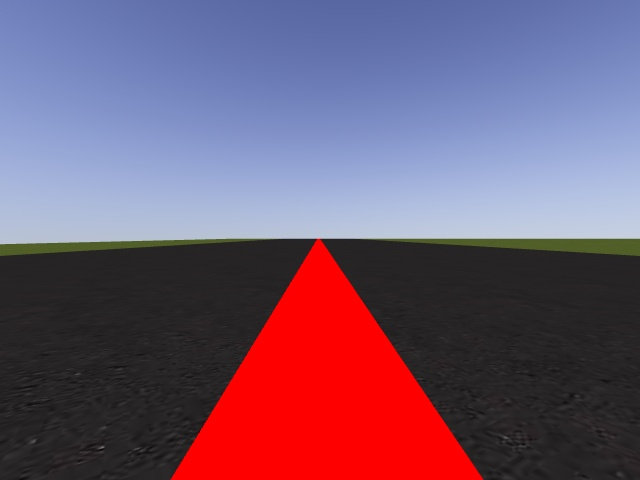
\includegraphics[width=0.4\columnwidth]{./figures/chapter_4/recta.jpg}
    \caption{
        \label{fig:simple-image}
            Imagen en bruto de la cámara del Fórmula-1.
    }
\end{figure}

Con la máscara obtenida se busca en diferentes filas el valor positivo ($255$) inicial y final para restarlos y obtener el centro de cada una de ellas. Esto retorna un valor (en píxeles) de la posición del centro en la imagen de entrada. Puede verse un ejemplo  de los estados simplificados para uno y tres percepciones en las figuras \ref{fig:estados-simplificados-1} y \ref{fig:estados-simplificados-3}.\\


\begin{figure}[ht!]
  \begin{center}
    \subfloat[1 puntos de percepción.]{\label{fig:estados-simplificados-1}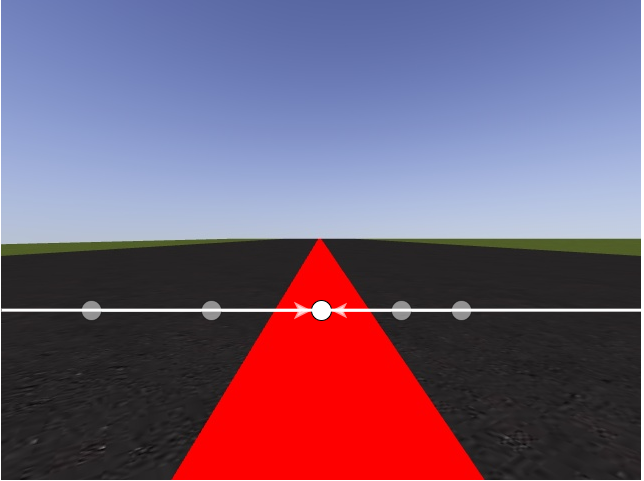
\includegraphics[width=.45\linewidth]{figures/chapter_4/estados_simplificados_1.png}}
    \hspace{0.1cm}
    \subfloat[3 puntos de percepción.]{\label{fig:estados-simplificados-3}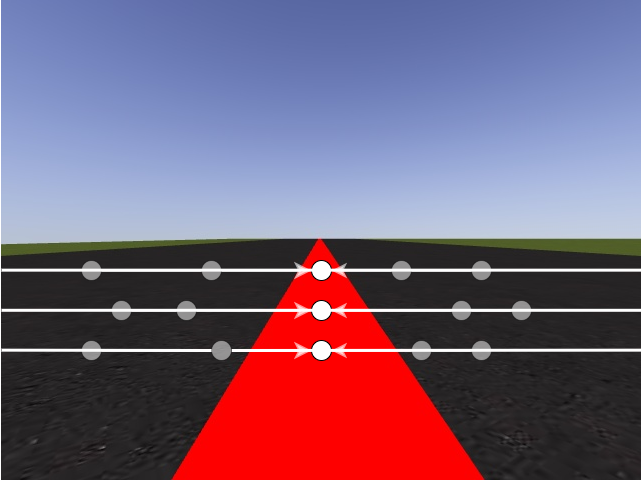
\includegraphics[width=.45\linewidth]{figures/chapter_4/estados_simplificados_3.png}}
  \end{center}
  \centering
  \captionsetup{justification=centering,margin=2cm}
  \caption{Diferentes puntos de percepción.}
  \label{fig:robots-gym-gazebo}
\end{figure}


Para evaluar la diferencia entre el valor observado del centro y el deseado se crea una plantilla que divide el espacio de la imagen en diferentes sectores, del 1 al 8 en valores positivos y negativos (figura \ref{fig:pipeline-procesamiento}). Esta rejilla servirá para generar un valor de <<posición>> del centro de la línea roja dentro de la imagen. Así pues, si un valor del centro cae en la región 4, el valor que devuelve todo el procesamiento será $4$ en vez del número de la columna del píxel de la imagen. El motivo de esta simplificación es reducir los valores de píxeles a un subconjunto simplificado que permita al algoritmo de aprendizaje por refuerzo encontrar una relación entre los valores de manera más rápida.\\

Como estados posibles para el algoritmo de aprendizaje se van a probar tres configuraciones: tomando la posición del centro en una sola fila de la imagen (un punto de percepción único), en dos (dos puntos de percepción) y en tres (tres puntos de percepción). En ese valor único, doble o triple se resume completamente la imagen de entrada, puesto que condensa la información necesaria para seguir la línea.\\

Por tanto, si tomamos la percepción simplificada usando únicamente una fila, el número de posiciones en los que puede estar el centro de la línea será de 17 (de $-8$ a $8$ contando el $0$) por el número de acciones que tenga el conjunto de estudio (3, 5 o 7) por el número de percepciones. Destacar que la gran mayoría no pueden darse por las limitaciones que ofrece la disposición de la línea sobre la imagen y la condición inicial que plantea el problema: seguir la línea. Puede verse en la figura \ref{fig:pipeline-procesamiento} la secuencia de procesamiento sobre la imagen de entrada hasta la salida para un punto de percepción.

\begin{figure}[!ht]
    \centering 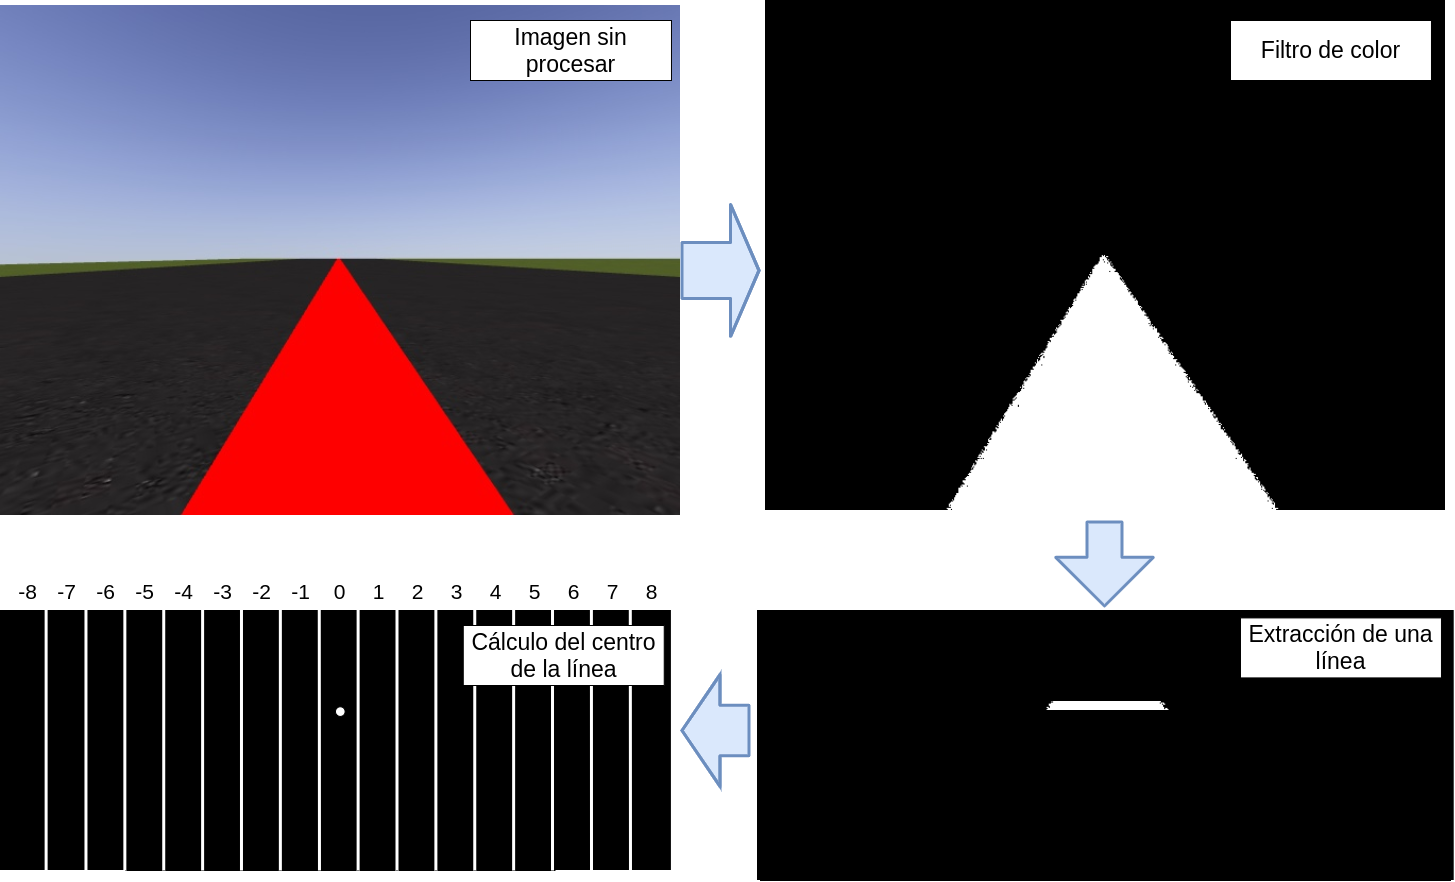
\includegraphics[width=1\columnwidth]{./figures/chapter_4/pipeline-procesamiento.png}
    \caption{
        \label{fig:pipeline-procesamiento}
            Cadena de procesamiento para un punto de percepción.
    }
\end{figure}

Para estados con dos o tres puntos de percepción se obtiene el valor central de la segmentación de la línea en dos o tres filas de la imagen de modo similar. De esta manera el estudio del comportamiento del agente será igual en todos los casos, como puede verse en la figura \ref{fig:pipeline-procesamiento-tres-puntos}.\\

\begin{figure}[!ht]
    \centering 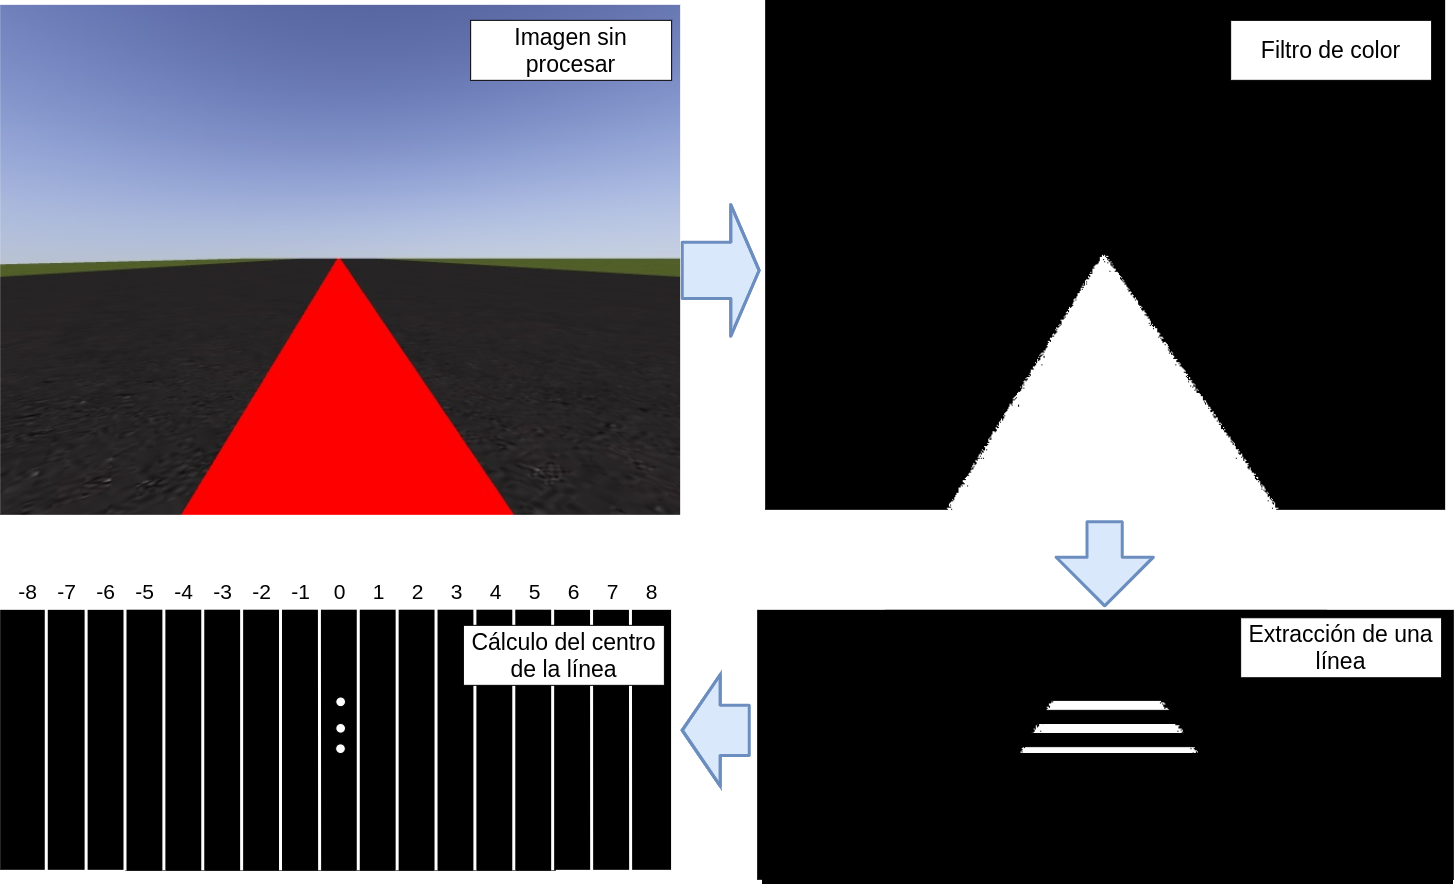
\includegraphics[width=1\columnwidth]{./figures/chapter_4/pipeline_3_puntos.png}
    \caption{
        \label{fig:pipeline-procesamiento-tres-puntos}
            Cadena de procesamiento para tres puntos de percepción.
    }
\end{figure}

Los valores simplificados son devueltos en forma de lista de enteros de Python constituyendo así los \textit{estados}. Esta lista de estados contiene el número de \textit{situaciones} a las que se enfrenta el algoritmo dada una imagen. Un ejemplo del resultado de esta sección puede verse en la figura \ref{fig:ejemplo-ejecucion} donde el resultado de ese estado corresponde con la secuencia $[1, 1, 0]$ en orden descendente.\\

\begin{figure}[!ht]
    \centering 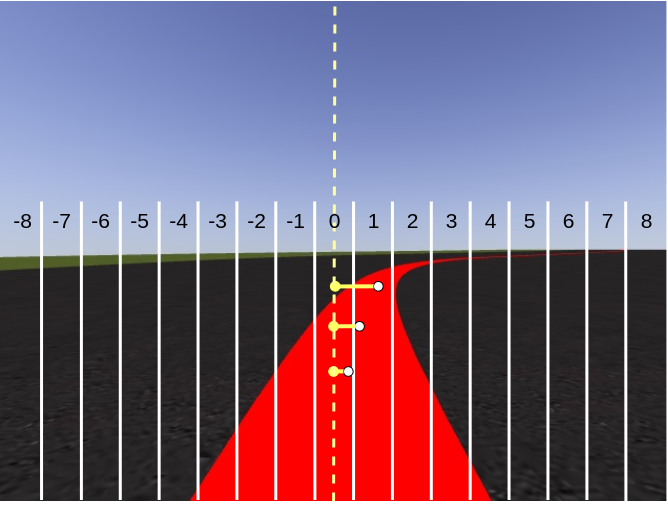
\includegraphics[width=0.5\columnwidth]{./figures/chapter_4/ejemplo_ejecucion.png}
    \caption{Ejemplo de estados retornados dado un paso.}\label{fig:ejemplo-ejecucion}
\end{figure}

De manera similar a como aprende el ser humano, cuanto más tiempo de entrenamiento se dedique a una tarea, más <<estados>> se verán y más experiencia se adquiere. A estados nunca vistos el comportamiento será impredecible.


%%%%%%%%%%%%%%%%%%%%%%%%%%%%%%%%%%%%%%%%%%%%%%%%%%%%%%%%%%%%%%%%%%%%%%%%%%%%%%%%%%%%%%%%%%%%%%%%%%%%%%%%%%%%%%%%
\subsection{Conjunto de acciones posibles}\label{conjunto-acciones}

Las acciones es otro de los grandes pilares del aprendizaje por refuerzo. En función de la situación en la que se encuentre el agente se tomará una u otra acción para corregir la dirección (inicialmente de manera aleatoria). En un entorno real, el conjunto de acciones tiene un espacio continuo de posibilidades. Pueden hacerse modificaciones infinitamente pequeñas para corregir la desviación cuando se conduce por una carretera o cuando se corrige el manillar de una bici para mantenerla en equilibrio. En el caso de este Trabajo Fin de Máster se seleccionan tres conjuntos de acciones discretas suficientes como para que el coche pueda completar todas las curvas del circuito.\\

Un conjunto tiene tres acciones posibles (tabla \ref{conjunto-1}), otro tiene 5 acciones posibles (tabla \ref{conjunto-2}) y el tercero contiene 7 acciones posibles (tabla \ref{conjunto-3}).\\

Para encontrar el conjunto que mejor resuelve el problema se crean estos tres repertorios, cada uno más complejo que el anterior. En la tabla \ref{conjunto-1} puede verse la distribución para el conjunto <<simple>> de acciones, únicamente dos valores de giro y uno de velocidad lineal.

\begin{table}[ht!]
\centering
\begin{tabular}{|l|c|c|c|}
\hline
\rowcolor[HTML]{EFEFEF} 
\textbf{Acción}                                       & \textbf{0} & \textbf{1} & \textbf{2} \\ \hline
\cellcolor[HTML]{EFEFEF}\textbf{V. Lineal $(m/s)$}    & 3          & 2          & 2          \\ \hline
\cellcolor[HTML]{EFEFEF}\textbf{V. Angular $(rad/s)$} & 0          & 1          & -1         \\ \hline
\end{tabular}
\caption{Conjunto simple.}\label{conjunto-1}
\end{table}

Aumentando ligeramente la dificultad, se añaden dos acciones más de velocidad angular para cubrir casos en los que las curvas puedan ser más cerradas. Es un conjunto <<medio>> de acciones. Puede verse esta distribución en la tabla \ref{conjunto-2}.

\begin{table}[]
\centering
\begin{tabular}{|l|c|c|c|c|c|}
\hline
\rowcolor[HTML]{EFEFEF} 
\textbf{Acción}                                       & \textbf{0} & \textbf{1} & \textbf{2} & \textbf{3} & \textbf{4} \\ \hline
\cellcolor[HTML]{EFEFEF}\textbf{V. Lineal $(m/s)$}    & 3          & 2          & 2          & 1          & 1          \\ \hline
\cellcolor[HTML]{EFEFEF}\textbf{V. Angular $(rad/s)$} & 0          & 1          & -1         & 1.5        & -1.5       \\ \hline
\end{tabular}
\caption{Conjunto medio.}\label{conjunto-2}
\end{table}

Por último, se reasignan valores y se añaden dos más, para casos todavía más extremos y que requieran de más velocidad angular. Este conjunto de acciones ya cuenta con 7 y se denomina <<dificil>>. Pueden verse los valores en la tabla \ref{conjunto-3}.

\begin{table}[ht!]
\centering
\begin{tabular}{|l|c|c|c|c|c|c|c|}
\hline
\rowcolor[HTML]{EFEFEF} 
\textbf{Acción}                                       & \textbf{0} & \textbf{1} & \textbf{2} & \textbf{3} & \textbf{4} & \textbf{5} & \textbf{6} \\ \hline
\cellcolor[HTML]{EFEFEF}\textbf{V. Lineal $(m/s)$}    & 3          & 2          & 2          & 1.5        & 1.5        & 1          & 1          \\ \hline
\cellcolor[HTML]{EFEFEF}\textbf{V. Angular $(rad/s)$} & 0          & 1          & -1         & 1          & -1         & 1.5        &  -1.5          \\ \hline
\end{tabular}
\caption{Conjunto difícil.}\label{conjunto-3}
\end{table}

Para la selección de los valores concretos de $v$ y $w$ para cada acción se ha ejecutado una solución al problema utilizando un algoritmo creado manualmente y se han comprobado los valores máximos alcanzados de giro para tener uno representativo que pueda solucionar la dificultad más extrema.



%%%%%%%%%%%%%%%%%%%%%%%%%%%%%%%%%%%%%%%%%%%%%%%%%%%%%%%%%%%%%%%%%%%%%%%%%%%%%%%%%%%%%%%%%%%%%%%%%%%%%%%%%%%%%%%%
\subsection{Función de recompensa}\label{funcion-recompensa}

Para completar un \textit{paso} (o \textit{step}) en el aprendizaje por refuerzo se necesita disponer de una función de recompensa que materialice numéricamente los valores retornados de la imagen procesada en un valor que sirva de guía para que la acción elegida como respuesta se repita o se evite.\\

En el punto \ref{percepcion-simplificada} se describían los pasos hasta obtener el centro de la línea. Para el cálculo de la recompensa se utiliza la diferencia entre ese valor central de la línea y el centro de la imagen (corresponde con el valor de píxel $320$ dado que la imagen es de $640$ píxeles de ancho). En función de la distancia que haya al centro se calcula la recompensa de regreso.\\

Al igual que ocurre con la percepción simplificada, se le otorga al robot cierta holgura o rango para fijar una recompensa. El objetivo es que el coche haga coincidir su centro con el centro de la línea por lo que en ese punto y sus cercanías la recompensa será máxima. Un poco más lejos la recompensa será un valor mediano y aún más lejos un último rango donde la recompensa será mínima pero aún válida. En otro caso, el episodio termina y reinicia la simulación. Los valores de recompensa usados en este trabajo pueden verse en la figura \ref{fig:valores-recompensa} recuadrados. El código de colores representa cómo de buena es la posición del centro en la imagen, siendo el verde muy buena, la amarilla un punto intermedio y la naranja un rango bajo. El color rojo se reserva para el rango no válido.\\

\begin{figure}[!ht]
    \centering 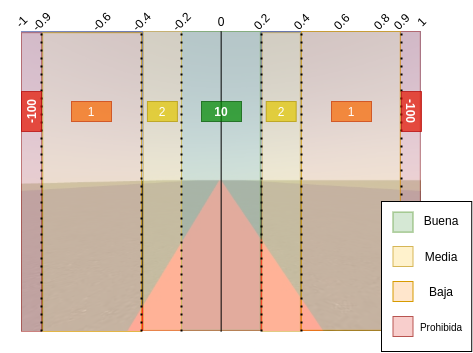
\includegraphics[width=0.7\columnwidth]{./figures/chapter_4/reward_distribution.png}
    \caption{
        \label{fig:valores-recompensa}
            Distribución de los valores de recompensa.
    }
\end{figure}

Mientras el agente mantenga el centro de la parte delantera dentro del rango válido ($[-0.9, 0.9]$) en la imagen se irán dando pequeños pasos (\textit{steps}) en el circuito siguiendo el algoritmo planteado en el punto \ref{qlearning}. En el momento que el centro de la línea segmentada supere los valores admitidos ($centro > 0.9$) se da por terminado el \textit{episodio} y se \textit{reinicia la simulación}.

%%%%%%%%%%%%%%%%%%%%%%%%%%%%%%%%%%%%%%%%%%%%%%%%%%%%%%%%%%%%%%%%%%%%%%%%%%%%%%%%%%%%%%%%%%%%%%%%%%%%%%%%%%%%%%%%
\subsection{Aprendizaje y ajustes}

Durante esta sección se han ido viendo las distintas partes de las que está compuesto el algoritmo que soluciona el problema planteado utilizando aprendizaje por refuerzo. En este punto se agrupan todas esa partes para entender la relación entre ellas y los resultados que devuelve. También se extrae conocimiento del comportamiento que sigue el coche durante el entrenamiento que aporta al desarrollador información <<psicológica>> para afinar los  parámetros del aprendizaje.\\

Siguiendo el flujo del programa en un entrenamiento se detallan algunos de los comportamientos derivados de la configuración y que han sido resueltos mediante iteraciones para el ajuste de los parámetros y de las condiciones del entrenamiento.\\

Cuando el entrenamiento empieza y se establece la comunicación con los componentes ROS y Gazebo, comienza un episodio dentro de un bucle \texttt{for} de Python. El comienzo de un episodio consiste en reiniciar la posición del robot y tomar una imagen de inicio, para tener un estado inicial con el que tomar decisiones. Siguiendo el paralelismo con una situación real es despertar o abrir los ojos y analizar lo primero que se ve. Seguidamente entra en otro bucle que son los \textit{pasos} o \textit{steps} y que se pasan a detallar a continuación:\\

\begin{enumerate}
    \item Se selecciona una acción del conjunto disponible. Inicialmente aleatoria y según va avanzando el programa se empiezan a seleccionar de la Tabla-Q que se está confeccionando.\\
    \item Se ejecuta el método \texttt{step} que recibe una acción:\\
    \begin{itemize}
        \item \textbf{Se convierte la acción en movimiento del robot}: Tomando los valores registrado de cada acción en forma de velocidad lineal y angular que se entregan a ROS y se ejecutan en el robot dentro del simulador Gazebo.\\
        \item \textbf{Se toma un fotograma de la cámara}: Esta imagen representa el estado $s+1$. La acción que se convierte en reacción en el robot ya ha sido procesada en el comienzo del episodio.\\
        \item \textbf{Se procesa la imagen obteniendo el centro de la línea}. Este punto guarda una característica muy interesante del comportamiento del agente. La altura seleccionada para calcular el centro de la línea (más cerca del horizonte o del robot) repercute en el comportamiento del agente, por lo que se ha seleccionado un valor que guarda un compromiso entre la posición del vehículo con respecto a la línea y la resolución del problema.\\
        
        Alturas por encima de la elegida (parte superior de la línea roja o el horizonte) hacen que el agente se quede muy separado de la línea roja sobre el asfalto, pegándose a las paredes como puede verse en la figura \ref{fig:distanciamiento-1}. Por el contrario, alturas inferiores hacen que el comportamiento sea muy agresivo dado que los puntos que están más cerca de la cámara se mueven más rápido. Idealmente, el punto inferior sería el que hay que seguir dado que coloca el vehículo justo encima de la línea pero implica que el entrenamiento no se complete. Esta altura intermedia permite mantener el coche cerca de la línea roja a la vez que completa entrenamientos.
        
        \begin{figure}[ht!]
            \centering 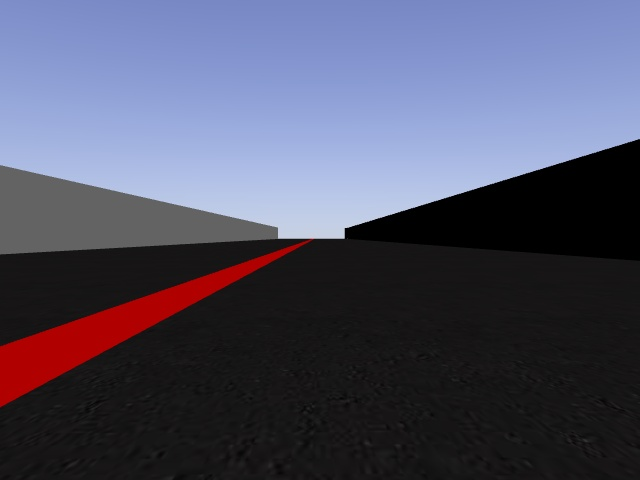
\includegraphics[width=0.5\columnwidth]{./figures/chapter_4/ataque_recta.jpg}
            \caption{Valores de centro de la línea cerca del horizonte.}\label{fig:distanciamiento-1}
        \end{figure}
        
        \item \textbf{Cálculo del valor de recompensa}: en función de la posición del centro de la línea y el centro de la imagen se retorna una recompensa mayor o menor (explicado en esta sección).\\
        \item \textbf{Se retorna al programa principal}: los valores del estado o percepción simplificada (vistos en la sección \ref{percepcion-simplificada}), la recompensa y el booleano \texttt{done}, que indica si este cálculo del centro ha sido exitoso, es decir, se encuentra dentro del rango permitido. Un valor de esta variable negativo (\texttt{False}) reiniciaría la simulación (el coche se ha salido de la línea).\\
    \end{itemize}
    \item Se agrega la recompensa a la variable de recompensa acumulada. Un valor muy alto de esta variable indica que el coche ha ido la mayor parte del entrenamiento con el morro y el centro de la línea alineados, es decir, ha conseguido la recompensa máxima en cada paso. Un valor menor indica que el agente ha estado oscilando en torno al centro, probando las áreas que retornan menor recompensa.\\
\end{enumerate}


El resultado final del entrenamiento es un modelo en formato de diccionario de Python que contiene los pares (\textit{estado, acción}) como clave y la recompensa como valor. Puede verse un ejemplo de la Tabla-Q para un conjunto de acciones simple (3 acciones) en la tabla \ref{tabla-q}.

\begin{table}[ht!]
\centering
\begin{tabular}{|c|c|}
\hline
\rowcolor[HTML]{C0C0C0} 
\textbf{(estado, acción)} & \textbf{Recompensa} \\ \hline
(4, 2)                     & 2                   \\ \hline
(-1, 0)                    & 63                  \\ \hline
(-5, 0)                    & -62                \\ \hline
(3, 2)                     & 32                  \\ \hline
\end{tabular}
\caption{Extracto de una Tabla-Q.}\label{tabla-q}
\end{table}

A la vista de los resultados del extracto de la Tabla-Q puede verse cómo un par (\textit{estado, acción}) que representa la situación de casi ir en la línea recta implica tomar la acción de ir recto. Es el caso de la segunda fila de la tabla: $(-1, 0)$ que devuelve una recompensa relativamente alta. Por el contrario, valores de (\textit{estado, acción}) como el de la fila tres ($-5,0$) devuelve una recompensa negativa dado que este conjunto significa haber ido recto cuando el punto estaba en una curva o se había producido una corrección. Es un estado que se quiere evitar y por eso el algoritmo la registra con un valor negativo. Comportamientos intermedios como la última fila ($3, 2$) devuelve recompensas intermedias donde si el centro se encuentra en un cuarto de la imagen se debe tomar la acción 2, girar a la derecha para corregir la desviación. Un estado muy parecido es la fila uno ($4,2$) pero puede verse cómo el algoritmo intentará no hacer demasiado caso a ese conjunto dado que la recompensa es muy pobre.\\

Un elemento importante que mejora la calidad y velocidad de entrenamiento han sido los \textit{saltos aleatorios} por cada reinicio del episodio. En la sección \ref{adaptacion-gym-gazebo} se vieron los puntos en los que el agente se posiciona al azar cuando se reinicia el episodio. Colocar al agente en estos sitios repercute en la velocidad a la que se rellena la Tabla-Q dado que los estados que únicamente podría ver al final del recorrido los está viendo al principio del entrenamiento. Con unos pocos reinicios, el agente ya dispone de un tamaño mínimo de la Tabla-Q para poder sobrevivir durante más tiempo en cada nuevo episodio.\\

En este capítulo se han visto detalladamente cada uno de los puntos que influyen en el entrenamiento de un agente en un entorno simulado utilizando el aprendizaje por refuerzo con el algoritmo Q-Learning. Una vez realizados la batería de experimentos se analizan los resultados para conocer en qué situaciones se comporta mejor y peor el agente aprendido.